\documentclass{article}
\usepackage{pgfplots}
\usepackage{amsmath}


\begin{document}
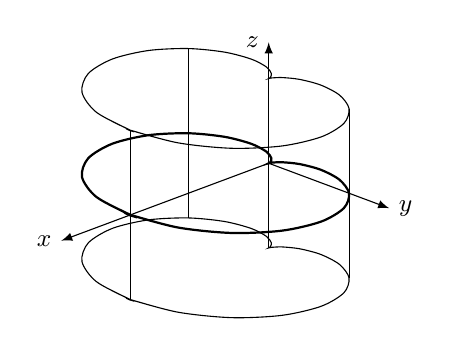
\begin{tikzpicture}[font=\small,declare function={fr(\t)=1+cos(\t);}]
\pgfmathsetmacro{\ta}{0}
\pgfmathsetmacro{\tb}{90}
\pgfmathsetmacro{\tc}{180}
\pgfmathsetmacro{\td}{270}
\pgfmathsetmacro{\h}{1.75}
\begin{axis}[axis lines=center,view/h=135,xtick={\empty},ytick={\empty},ztick={\empty},xlabel={$x$},ylabel={$y$},zlabel={$z$},xlabel style={anchor=east},ylabel style={anchor=west},zlabel style={anchor=east},enlargelimits=true, axis x line=none,axis y line=none, axis z line=none]
\addplot3[smooth,thick,data cs=polar,domain=0:360](\x,{fr(\x)},0);
\addplot3[smooth,data cs=polar,domain=0:360](\x,{fr(\x)},-\h);
\addplot3[smooth,data cs=polar,domain=0:360](\x,{fr(\x)},\h);
\addplot3[data cs=polar]coordinates {(\ta,{fr(\ta)},-\h)(\ta,{fr(\ta)},\h)};
\addplot3[data cs=polar]coordinates {(\tb,{fr(\tb)},-\h)(\tb,{fr(\tb)},\h)};
\addplot3[data cs=polar]coordinates {(\tc,{fr(\tc)},-\h)(\tc,{fr(\tc)},\h)};
\addplot3[data cs=polar]coordinates {(\td,{fr(\td)},-\h)(\td,{fr(\td)},\h)};
\addplot3[-latex]coordinates{(0,0,0)(3,0,0)}node[left]{$x$};
\addplot3[-latex]coordinates{(0,0,0)(0,1.5,0)}node[right]{$y$};
\addplot3[-latex]coordinates{(0,0,0)(0,0,2.5)}node[left]{$z$};
\end{axis}
\end{tikzpicture}
\end{document}
